\documentclass{article}

% Recommended, but optional, packages for figures and better typesetting:
\usepackage{microtype}
\usepackage{graphicx}
\usepackage{subfigure}
\usepackage{booktabs} % for professional tables

% hyperref makes hyperlinks in the resulting PDF.
% If your build breaks (sometimes temporarily if a hyperlink spans a page)
% please comment out the following usepackage line and replace
% \usepackage{icml2021} with \usepackage[nohyperref]{icml2021} above.
\usepackage{hyperref}
\usepackage{xr}
\externaldocument{blind_denoising}
% Attempt to make hyperref and algorithmic work together better:
\newcommand{\theHalgorithm}{\arabic{algorithm}}

% Use the following line for the initial blind version submitted for review:
\usepackage{icml2021}

% custom packages
\usepackage{amsmath}
\usepackage{amssymb}
% for referencing footnotes several times. to load after hyperref
\usepackage{cleveref}
\crefformat{footnote}{#2\footnotemark[#1]#3}
% \usepackage{times}
% \usepackage{epsfig}
% If accepted, instead use the following line for the camera-ready submission:
%\usepackage[accepted]{icml2021}

% The \icmltitle you define below is probably too long as a header.
% Therefore, a short form for the running title is supplied here:
\icmltitlerunning{SI for Joint self-supervised blind denoising and noise estimation}
\newcommand{\interval}[2]{\mathopen{[}#1\,;#2\mathclose{]}}
\renewcommand{\thetable}{S\arabic{table}}
\renewcommand{\thefigure}{S\arabic{figure}}
\renewcommand{\thesection}{S\arabic{section}}
% \newcommand{\beginsupplement}{
%  }

\begin{document}
\twocolumn[
\icmltitle{Supplementary information for Joint self-supervised blind denoising and noise estimation}

\icmlsetsymbol{equal}{*}

\begin{icmlauthorlist}
\icmlauthor{Jean Ollion}{sabilab}
\icmlauthor{Charles Ollion}{cmap}
\icmlauthor{\'Elisabeth Gassiat}{ups}
\icmlauthor{Sylvain Le Corff}{tsp,cmap}
\icmlauthor{Luc Leh\'ericy}{uca}
\end{icmlauthorlist}

\icmlaffiliation{sabilab}{SABILab, Die, France}
\icmlaffiliation{cmap}{CMAP, Ecole Polytechnique, Institut Polytechnique de Paris, France}
\icmlaffiliation{tsp}{Samovar, T\'el\'ecom SudParis, D\'epartement CITI, Institut Polyechnique de Paris, France}
\icmlaffiliation{ups}{Universit\'e Paris-Saclay, CNRS, Laboratoire de math\'ematiques d'Orsay, 91405, Orsay, France}
\icmlaffiliation{uca}{Laboratoire J. A. Dieudonn\'e, Universit\'e C\^ote d'Azur, CNRS, 06108, Nice, France}

\icmlcorrespondingauthor{Jean Ollion}{jean.ollion@polytechnique.org}
\icmlcorrespondingauthor{Sylvain Le Corff}{sylvain.le_corff@telecom-sudparis.eu}

\icmlkeywords{Blind Denoising, Self-supervised, Bio-image, Machine Learning}

\vskip 0.3in
]

\section{Additional Implementation details}
\label{si:implementation}
\subsection{Networks and training}
\paragraph{D-Net architecture details.}
The architecture is based on U-net \cite{ronneberger2015u}.
We propose several changes from the original version: we do not crop the image and use zero-padding instead, we use 2 levels of contractions/expansions with 64 filters, expansions are performed by an upsampling layer with nearest-neighbor approximation directly followed by 2x2 convolution. We also add two layers of 1x1 convolution with 64 filters and ReLU activation at the end of the network, and set no activation function at the output layer.

\paragraph{N-Net architecture details.}
In the case of a Gaussian noise, the N-Net is composed 3 successive blocks, each block being composed of two 1x1 convolutions layers of 64 filters, each followed by a non-linear activation layer (alternatively tanh and leaky ReLU with alpha parameter set to $0.1$). A convolution 1x1 with a single channel followed by an exponential activation function is placed after the last block (to ensure that the predicted $\sigma$ is positive).

In the case where the N-net predicts a GMM with N components with weights $(\alpha_i)_{1\leqslant i\leqslant N}$, means $(\mu_i)_{1\leqslant i\leqslant N}$ and variances $(\sigma^2_i)_{1\leqslant i\leqslant N}$, the second block is connected to three distinct blocks, each connected to a convolution 1x1 with:
\begin{itemize}
  \item N channels, followed by an exponential activation function to predict $\sigma_{i}$.
  \item N channels, followed by a softmax activation to predict $\alpha_{i}.$\footnote{When $N=2$, only one channel is used and followed by a sigmoid activation function.}
  \item N-1 channels to predict the ditribution means $\mu_{i}$.
\end{itemize}
To ensure that the distribution is centered, the center of the last distribution is computed as
$$
\mu_{N} = \frac{1}{\alpha_{N-1}} \sum_{i=1}^{N-1}{\alpha_{i} \mu{i}}\,.
$$

\section{Datasets}
\subsection{Experimental Datasets}
\label{si:datasetxp}
\paragraph{Datasets published along with the PN2V \cite{krull2019probabilistic}.}
\begin{itemize}
  \item \emph{Convallaria} dataset, referred to as \emph{PN2V-C} is composed of 100 images of size $1024$x$1024$. Evaluation subset is: $(Y, X)\in(\interval{0}{512}, \interval{0}{512})$
  \item \emph{Mouse skull nuclei} referred to as \emph{PN2V-MN} is composed 200 images of size $512$x$512$. Evaluation subset is: $(Y, X)\in(\interval{0}{512}, \interval{0}{256})$
  \item \emph{Mouse Actin} referred to as \emph{PN2V-MA} is composed of 100 images of size $1024$x$1024$. Evaluation subset is: $(Y, X)\in(\interval{0}{1024}, \interval{0}{512})$
\end{itemize}

The \emph{PN2V-C} and \emph{PN2V-MA} datasets are acquired on a spinning disc confocal microscope and \emph{PN2V-MN} dataset is acquired with a point scanning confocal microscope.
Datasets can be downloaded from: \url{https://github.com/juglab/pn2v}

\paragraph{Datasets published in \cite{zhou2020w2s}.}

We used the 16-bit raw images kindly provided by the authors.
The dataset is composed of 120 FOV of 400 observations of size $512$x$512$ pixels.
The first 80 are used for training and the last 40 for evaluation.
Following the authors, for each FOV, only the observation of index 249 is used for training and evaluation
images are acquired with a electron-multiplying charge-coupled device camera on a wide-field microscope.
It can be downloaded here: \url{https://datasets.epfl.ch/w2s/W2S_raw.zip}

\paragraph{Normalization.}

For both datasets images were normalized using the modal value as center and the difference between modal value and $95\%$ percentile as scale factor, computed on the whole dataset.
This is relevant in fluorescence microscopy data where signal is often less abundant than background with proportion that vary among images and signal distribution often has a heavy tail towards high values.

For the 6 datasets, images are encoded in 16-bit thus the actual data range of each ground truth image is used for PSNR and SSIM computation.

\subsection{Synthetic noise datasets}
\label{si:synthetic}
\begin{itemize}
  \item Additive gaussian: $Y = X + \varepsilon$ with $\varepsilon \sim \mathcal{N}(0, \sigma^2)$, $\sigma=20$.
  \item Poisson-Gaussian: $Y = X + (\alpha * (X-\underline{X}) + \eta^2 )^{1/2}\varepsilon$  with $\varepsilon \sim \mathcal{N}(0, 1)$, $\alpha=5, \eta=12$ and $\underline{X}$ being the minimal value of the ground truth on the whole dataset.
  \item Speckle: $X = X + (X-min(\underline{X}))\varepsilon$  with $\varepsilon \sim \mathcal{N}(0, \sigma^2)$, $\sigma=0.405$ and $\underline{X}$ being the minimal value of the ground truth on the whole dataset.
\end{itemize}

\section{Noise estimation}
\label{si:skewness}
\begin{figure}[ht]
\begin{center}
\centerline{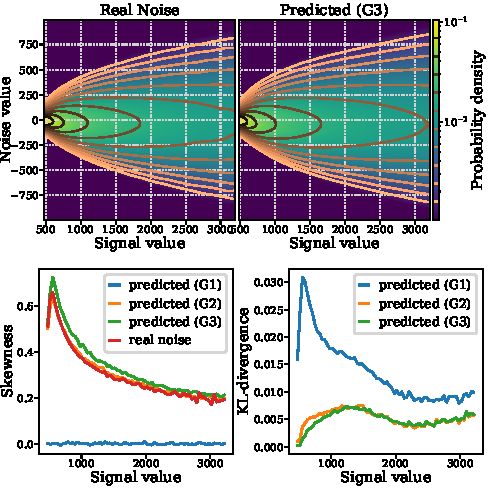
\includegraphics[width=\columnwidth]{fig_skewness_pn2v-C.pdf}}
\caption{Real noise estimation for dataset \textit{PN2V-C}. See main text Fig~\ref{fig:skewness}.
}
\end{center}
\vskip -0.2in
\end{figure}

\begin{figure}[ht]
\begin{center}
\centerline{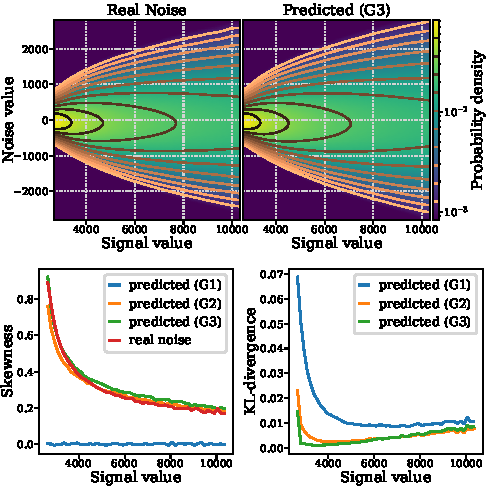
\includegraphics[width=\columnwidth]{fig_skewness_pn2v-MN.pdf}}
\caption{Real noise estimation for dataset \textit{PN2V-MN}. See main text Fig~\ref{fig:skewness}.
}
\end{center}
\vskip -0.2in
\end{figure}

\begin{figure}[ht]
\begin{center}
\centerline{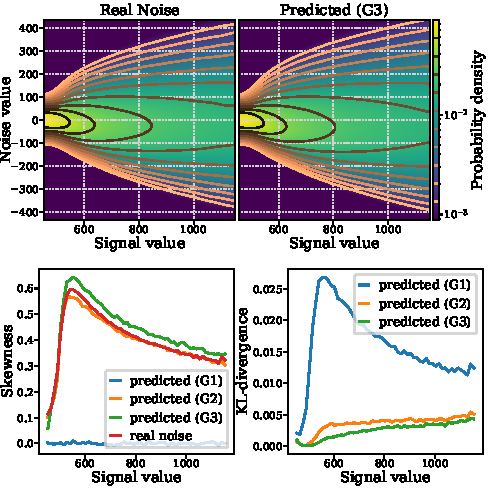
\includegraphics[width=\columnwidth]{fig_skewness_pn2v-MA.pdf}}
\caption{Real noise estimation for dataset \textit{PN2V-MA}. See main text Fig~\ref{fig:skewness}.
}
\end{center}
\vskip -0.2in
\end{figure}

\begin{figure}[ht]
\begin{center}
\centerline{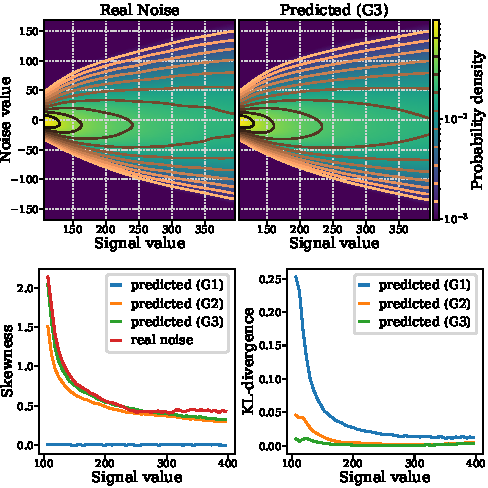
\includegraphics[width=\columnwidth]{fig_skewness_w2s-2.pdf}}
\caption{Real noise estimation for dataset \textit{W2S-2}. See main text Fig~\ref{fig:skewness}.
}
\end{center}
\vskip -0.2in
\end{figure}

\begin{figure}[ht]
\begin{center}
\centerline{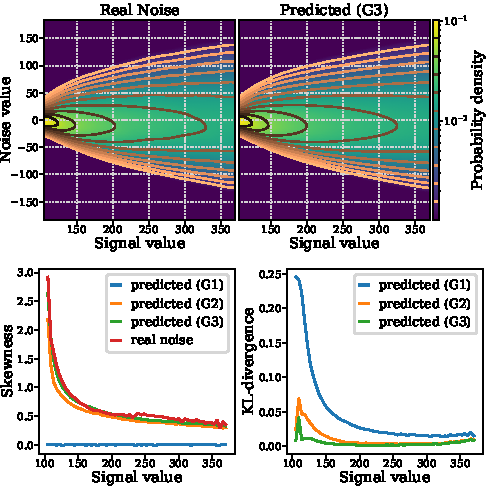
\includegraphics[width=\columnwidth]{fig_skewness_w2s-3.pdf}}
\caption{Real noise estimation for dataset \textit{W2S-3}. See main text Fig~\ref{fig:skewness}.
}
\end{center}
\vskip -0.2in
\end{figure}
\clearpage
{\small
\bibliography{blind_denoising}
\bibliographystyle{icml2021}
}
\end{document}
